\documentclass[12pt]{article}
\usepackage{graphicx} % Required for inserting images
\usepackage[a4paper,left=2cm,right=2cm,top=2.5cm,bottom=2.5cm]{geometry}
\usepackage[round]{natbib}
\usepackage{parskip}
\usepackage{amsmath}
\usepackage{mathtools} % allows \coloneq

% for tables
\usepackage{tabulary} % auto word wrap
\usepackage{booktabs} % toprule, midrule, bottomrule

% for links to figures, tables
\usepackage{hyperref}
\hypersetup{
    colorlinks   = true, %Colours links instead of ugly boxes
    urlcolor     = blue, %Colour for external hyperlinks
    linkcolor    = blue, %Colour of internal links
    citecolor   = blue %Colour of citations
}

\usepackage{xcolor}
\definecolor{maroon}{RGB}{153,0,51}
\definecolor{darkgreen}{RGB}{0,100,0}
\newcommand{\m}[0]{\color{maroon}}
\newcommand{\g}[0]{\color{darkgreen}}

% for smaller captions
\usepackage{caption}
\captionsetup{font=footnotesize}

% for annotated equations
% \usepackage{annotate-equations}

% for shaded-box results and remarks and examples
\usepackage{amsthm}
\usepackage{framed}

% for table of contents for supplement only
% \usepackage{minitoc}
% \renewcommand{\ptctitle}{} % No title "Table of Contents" for the toc
% \renewcommand \thepart{} % Make the "Part I" text invisible
% \renewcommand \partname{}
% \usepackage[toc,page,header]{appendix}

% ---------------------------------------------------------------------------------------
\title{Text of Working Papers and Information Papers from the Antarctic Treaty Consultative Meetings}
\author{Carlo H{\"a}m{\"a}l{\"a}inen, Zachary T. Carter, and Nadiah P. Kristensen}
%\date{September 2024}

\begin{document}
% ---------------------------------------------------------------------------------------
\maketitle

% suppress table of contents in main part
% \doparttoc % Tell to minitoc to generate a toc for the parts
% \faketableofcontents % Run a fake tableofcontents command for the partocs
% \part{} % Start the document part

% shaded-box results and remarks
\colorlet{shadecolor}{blue!3}
%
\newtheoremstyle{mystyle}%                % Name
  {}%                                     % Space above
  {}%                                     % Space below
  {}%                                     % Body font (often italic)
  {}%                                     % Indent amount
  {\bfseries}%                            % Theorem head font
  {.}%                                    % Punctuation after theorem head
  { }%                                    % Space after theorem head, ' ', or \newline
  {\thmname{#1}\thmnumber{ #2}\thmnote{ (#3)}}% % Theorem head spec (can be left empty, meaning `normal')
\theoremstyle{mystyle}
%
\newtheorem{res2}{Result}[section]
\newenvironment{res}
  {\begin{shaded}\begin{res2}}
  {\end{res2}\end{shaded}}
%
\newtheorem{rmk2}{Remark}[section]
\newenvironment{rmk}
  {\begin{shaded}\begin{rmk2}}
  {\end{rmk2}\end{shaded}}

% shaded examples
\theoremstyle{definition}
\newtheorem{examplex}{Example}
\newenvironment{exmi}
  {\pushQED{\qed}\renewcommand{\qedsymbol}{$\triangleleft$}\examplex}
  {\popQED\endexamplex}
\colorlet{shadecolor}{blue!3}
\newenvironment{exm}
  {\begin{shaded}\begin{exmi}}
  {\end{exmi}\end{shaded}}
% ---------------------------------------------------------------------------------------

\section{To do}

\begin{itemize}
    \item A section comparing Linux-tool results to AI OCR.
    \item Missing software citations
\end{itemize}

\section{Introduction}

The Antarctic Treaty System (ATS), founded on the Antarctic Treaty 1959, 
is a system of interlinked regulations and institutions that govern activities concerning Antarctica 
\citep{barrett2020antarctic}. 
Parties to the Treaty meet annually at the Antarctic Treaty Consultative Meetings (ATCMs) 
to exchange information, consult, and formulate measures 
to present to their governments in furtherance of the Treaty. 
The two main inputs to ATCMs are
Working Papers (WPs),
which must be discussed during the meeting
and decisions are made based on their recommendations;
and Information Papers (IPs),
which provide supplementary information to WPs and agenda items 
({\m cite}). %\citep{gardiner2025measuring} 
Consequently, WPs and IPs 
% represent a rich corpus for researchers 
% seeking to understand the evolution of 
% Antarctic policy, environmental management, and international cooperation. 
% and source of information 
provide a valuable material record of 
policy evolution and decision-making
% the evolution of Antarctic policy, environmental management, and international cooperation. 
over the ATS's history.

However,
researchers face two significant barriers to analysing ATCM documents:
their fragmented storage across multiple databases
and the poor-quality digitisation of older materials.
Most ATCM documents are available from the Antarctic Treaty System database (ATSD)
hosted by the Secretariat of the Antarctic Treaty; however, significant gaps in the collection exist. 
Most notably, some early-year WPs are missing,
and gaps are clustered in certain years.
A partially overlapping online database, 
the Antarctic Documents Database (ATADD) hosted by the University of Tasmania,
could potentially fill some of these gaps,
and a consolidated repository integrating both sources
would create a more accessible resource.

The variable quality of document digitisation 
impedes the use of modern text-analysis techniques,
such as natural language processing (NLP) or large language models,
% for topic modelling, sentiment analysis, or network analysis 
which require access to machine-readable text data. 
Middle-year documents are typically available as DOC files, which use a proprietary binary format that requires conversion for analysis. 
More problematically, early documents 
(particularly those from the 1960s--1980s)
exist primarily as scanned images of document pages embedded in PDFs,
which were often typewritten,
exhibit poor scan quality, 
and contain various imaging artefacts.
To extract machine-readable text from these early documents, researchers must rely on optical character recognition (OCR) technology. 
However, we have found that off-the-shelf free software (e.g., Tesseract) 
performs poorly on these materials, 
frequently producing text riddled with errors, missing passages, and formatting inconsistencies 
that render the output unsuitable for systematic analysis.

With the advent of multimodal AI models,
new opportunities have emerged for high-quality text extraction from challenging documents. 
These models can simultaneously process visual layout cues (e.g., formatting, tables, and positioning) alongside textual content, 
making them particularly well-suited to the complex layouts and variable quality typical of historical ATCM documents.

In this document, we present a comprehensive dataset that addresses both challenges outlined above. 
We have collated all WPs and IPs available from the ATSD, 
filled gaps in this collection with WPs from the ATADD, 
and systematically extracted machine-readable text from all documents. 
For early documents requiring OCR, we employed a multimodal large language model, 
which produced significantly more accurate text extraction compared to traditional OCR software. 
The resulting dataset provides researchers with a consolidated, machine-readable corpus of ATCM documents spanning the Treaty's history.
%
We describe the methods used to create the dataset, 
discuss known limitations and ongoing quality issues, 
and provide guidance for accessing and using the content for research purposes.

\section{Methods}

Working Papers (WPs) and Information Papers (IPs) were obtained from two online databases:
the Antarctic Treaty System Database (ATSD) and the Antarctic Documents Database (ATADD).
%
The ATSD is hosted online by the Secretariat of the Antarctic Treaty,
and it is accessible at \url{https://www.ats.aq/}.
The website is the central digital archive and information hub for the Antarctic Treaty System (ATS),
and the Secretariat maintains it to fulfill its core mandate 
of collecting, storing, archiving and making available the documents of the Antarctic Treaty Consultative Meetings (ATCMs).
%
The ATADD is hosted online by the University of Tasmania,
and it is accessible at \url{https://www.utas.edu.au/library-resources/atadd}.
It is a comprehensive collection of Antarctic law and policy documents, 
assembled over decades by international lawyer Bill Bush.
In 2016, Bush's collection was given to Australian Antarctic scholar Andrew Jackson, 
and a Australian Research Council (ARC) grant made possible the digitisation of the entire collection.

The document collation was performed in two stages.
In the first stage,
we collated a list of WPs and IPs available from the ATSD,
which holds the most complete collection of documents.
In the second stage,
we identified gaps in the WP collection and supplemented them with documents from the ATADD where possible.
We chose to focus on WPs because of their central role as inputs to the ATCMs and decision-making processes.
We identified WP gaps by first finding gaps in the sequence of WP numbers,
and also by finding and consulting official document lists from ATCMs 
({\tt /data\_accountability/atadd\_utas\_database/list\_of\_docs}).

Our main concerns were coverage and data accountability.
To ensure full data coverage of the ATSD,
we used a metaprogramming approach to query the website and database,
which eliminated the need to manually discover their underlying structures,
reducing the possibilities for omissions and errors (Sect.~\ref{getting_from_ATSD}).
For data accountability,
we implemented a HTTP-response caching system,
which recorded the timestamps and full responses of each request (Sect.~\ref{http_cache}).
For the manual second stage,
we made a detailed record of how each missing WP was identified,
and we give our reasons for each gap that remains (Sect.~\ref{getting_from_ATADD}).

\subsection{Identifying documents in the Antarctic Treaty System database}
\label{getting_from_ATSD}

The Secretariat of the Antarctic Treaty provides a web interface for searching and retrieving documents 
(\url{https://www.ats.aq}).
When researchers access this database through a web browser, 
they interact with search forms containing dropdown menus, checkboxes, and text fields to specify their queries.
These forms are built from HTML code that defines their structure and appearance.
When a search is submitted, the website sends the query to the database server (ATSD), 
which returns matching documents and their metadata in structured formats (typically JSON).
For systematic analysis of Antarctic Treaty documents, manually performing these searches would be impractical and error-prone.
Writing code to `scrape' the website is also error-prone due to the need to manually decipher and reconstruct the structure
of both the HTML forms and the API responses 
(i.e., the JSON structured data returned by the database).
Instead, 
we used automated code generation to programmatically interact with the database
with built-in type safety and consistent reliability.

To ensure code safety and scientific reproducibility 
when accessing the ATSD search endpoints,
we implement a metaprogramming approach.
Metaprogramming means writing code that writes or manipulates other code. 
We used Goquery (a library that parses HTML),
together with Go's Abstract Syntax Tree (AST) library
(a tool that can generate Go source code)
to create metaprogramming tools 
that automatically parsed the website's HTML structure and API response formats
generating code that precisely matched the database's interface.
The code was type-save,
which means variable types are strictly enforced at compile time,
preventing incorrect usage.
By matching the database's interface,
we eliminated the need to manually define HTML form structures and API parameters
(the specific values used to query the database, e.g., meeting dates, document types).

Two automated tools were created 
to parse the database's web interface and API responses to generate strongly-typed Go code.
First, 
{\tt tools/metadata/main.go} scraped the search form's HTML elements 
(dropdown menus, radio buttons, and input fields) 
to automatically generate type-safe constants for search parameters like 
meeting types, document categories, and topic classifications.
Second, 
{\tt tools/structs/main.go} analysed JSON responses from the API 
to automatically infer and generate corresponding Go struct definitions, 
including proper type handling for nested objects and arrays. 

Our metaprogramming approach accounted for inconsistencies between interfaces.
For example, 
the Treaty Search Database uses date strings as keys for ATCMs, 
whereas the Meeting Documents Database uses sequential integers. 
Thus, ATCM I (Canberra 1961) is referred to by the key {\tt "07/24/1961"} in the Treaty Search Database, 
while the same meeting is referenced by the key {\tt "2"} in the Meetings Documents Database.
Without a metaprogramming approach, 
a researcher would need to manually discover this mapping and maintain it throughout their code,
risking errors when the database changes or when switching between search endpoints.
Instead, 
the metaprogramming tools automatically discovered this quirk by scraping both interfaces, 
generating separate types for each system that ensure proper referencing regardless of which endpoint is being queried.

The metaprogramming approach eliminates the risk of runtime errors from mistyped parameters or incorrect data structure assumptions,
while automatically adapting to changes in the database's schema without requiring manual code updates,
which ensures long-term research data reliability.
Instead of discovering errors like misspelled field names when the analysis crashes during execution, 
any mistakes are caught immediately when the code is compiled, before it ever runs. 
This eliminates an entire class of bugs that could occur at runtime.
Scientific reproducibility is enhanced because the data access layer perfectly matches the actual API structure. 
This prevents silent data corruption or analysis failures that might otherwise go undetected until much later stages of research. 
The strongly-typed code generation ensures that all database interactions are verified at compile time, creating a reliable foundation for downstream analysis.

Documents were often available in multiple languages, 
and a preference order was imposed: English, Spanish, French, Russian.
For example, if a document was only available in Spanish and Russian, then the Spanish version was downloaded. 

\subsection{Obtaining and recording Antarctic Treaty System database responses}
\label{http_cache}

A key challenge of using web-based data sources is ensuring reproducibility and traceability of the data.
To ensure data accountability,
we implemented a persistent HTTP response caching system ({\tt cache.go} module).
The cache recorded the full response from the Secretariat website.
including meta-data about when the ATSD (database) was accessed to discover the existence of each document.
This will allow future researchers to replicate our analysis using the database state as it existed at the time we accessed it.
When the database is updated or changed in the future, 
the exact nature of the change can be discovered by comparing its new state to the state that we recorded.

We created the HTTP response caching system using an SQLite database,
which had the practical benefit of ensuring the completeness of each transaction.
SQLite was selected as the persistent store because it implements ACID 
(Atomicity, Consistency, Isolation, Durability) properties, 
which are essential for scientific data integrity. 
These properties ensure that database transactions are processed reliably 
even during system failures or power outages. 
The ACID compliance guarantees that each database operation is treated as a single, indivisible unit
that either completely succeeds or completely fails, preserving data validity.
Each cache write operation begins with {\tt tx.Begin()} and must end with either
{\tt tx.Commit()} (success) or {\tt tx.Rollback()} (failure),
which creates an `all-or-nothing' boundary around the entire operation.
Before storing new data, 
the system checks if an entry already exists. 
If it finds conflicting data (different headers or body content), it raises an error and rolls back the transaction, 
preventing the storage of inconsistent information.
If anything goes wrong during the operation (e.g., network interruption, power failure, program crash),
the transaction is automatically rolled back, leaving the database in its original, consistent state.
Only after all validation passes does the system call {\tt tx.Commit()}, 
which atomically writes all changes to disk in a single operation that cannot be interrupted.
The transaction system ensures that the cache contains only complete, 
verified responses that can be trusted for reproducible research.
Each cached entry is either a perfect replica of what the server sent,
or it does not exist at all.

We designed the cache to 
transforms ephemeral web requests into a permanent, auditable scientific record.
Every HTTP request to the ATSD is automatically stored in a SQLite database with a precise timestamp.
This creates an immutable record of exactly when each piece of data was obtained, 
which is essential for documenting data collection methodology and detecting when source data might have changed.
The system stores not just the response body, but also HTTP headers, status codes, and complete metadata. 
This preserves the full context of each data retrieval, 
allowing researchers to verify that the cached data matches what was originally received from the server.
If the system attempts to cache a response that differs from a previously cached version of the same URL, 
it raises an error.
This prevents silent data corruption and alerts researchers when the source database has been updated.
Once cached, the system can serve identical responses without internet access,
enabling other researchers to reproduce analyses using the exact same data that was originally retrieved,
even if the online database has since changed.

A HTTP client was integrated with the cache 
to increase efficiency and be respectful of the Secretariat's servers.
When data is requested, the system first tries to obtain a response from the cache.
If the request is not already in the cache, the request is forwarded to the remote server,
which is then stored in the cache.
This allows one to use the data accumulated in the SQLite database as though it were a normal client.
The HTTP client serves as a centralised request coordinator 
that manages all communication with the Secretariat servers, 
allowing rate limiting and respectful data access patterns. 
Rather than allowing individual data collection processes 
to make uncontrolled requests 
that could overwhelm the Secretariat's infrastructure, 
the client acts as a throttling gateway 
that enforces appropriate delays between requests, 
respects server-indicated rate limits, 
and prevents the kind of aggressive scraping 
that could be seen as abusive or could trigger defensive measures from the target servers. 

\subsection{Identifying missing WPs available in the Antarctic Documents Database}
\label{getting_from_ATADD}

We identified WPs potentially missing from the ATSD, 
manually searched for them via the ATADD web portal,
and added their URL to the list of paper download links.
Unlike the ATSD above, it was not possible to automate this process,
and therefore we documented each step and decision made in 
the {\tt data\_accountability} directory.
The first and simplest indication that WP is missing is a gap in the sequential
WP numbering system,
and we used official document lists to distinguish between true gaps
and WP numbers that were not used
(available in ({\tt data\_accountability/atadd\_utas\_database/list\_of\_docs/}).
The document lists were obtained from ATADD,
and they often contained pencil annotations by Bill Bush, 
which were useful for identifying missing WPs (e.g., Fig.~\ref{bush_annotation}).
We found significant gaps in the years 1989, 1995, and 2001;
however, missing WPs from 2001 were not available on ATADD either.
A full accounting of each potentially missing WP is given in
{\tt data\_accountability/atadd\_utas\_database/wps\_missing.csv}
along with identifying information about WPs that remain missing
(e.g., title, list of authors).

\begin{figure}[h]
    \begin{minipage}[b]{0.50\textwidth}
        \caption{
        An example of an annotation added by Bill Bush
        to an official List of Working Papers for ATCM 22 (1998) obtained from ATADD.
        The annotation reads ``28, Argentina, Antarctic [illegible]''.
        This alerted us to the existence of a WP 28 that was missing from the ATSD,
        which we were able to find in the ATADD.
        } \label{bush_annotation}
    \end{minipage}
    \hfill
    \begin{minipage}[b]{0.45\textwidth}
        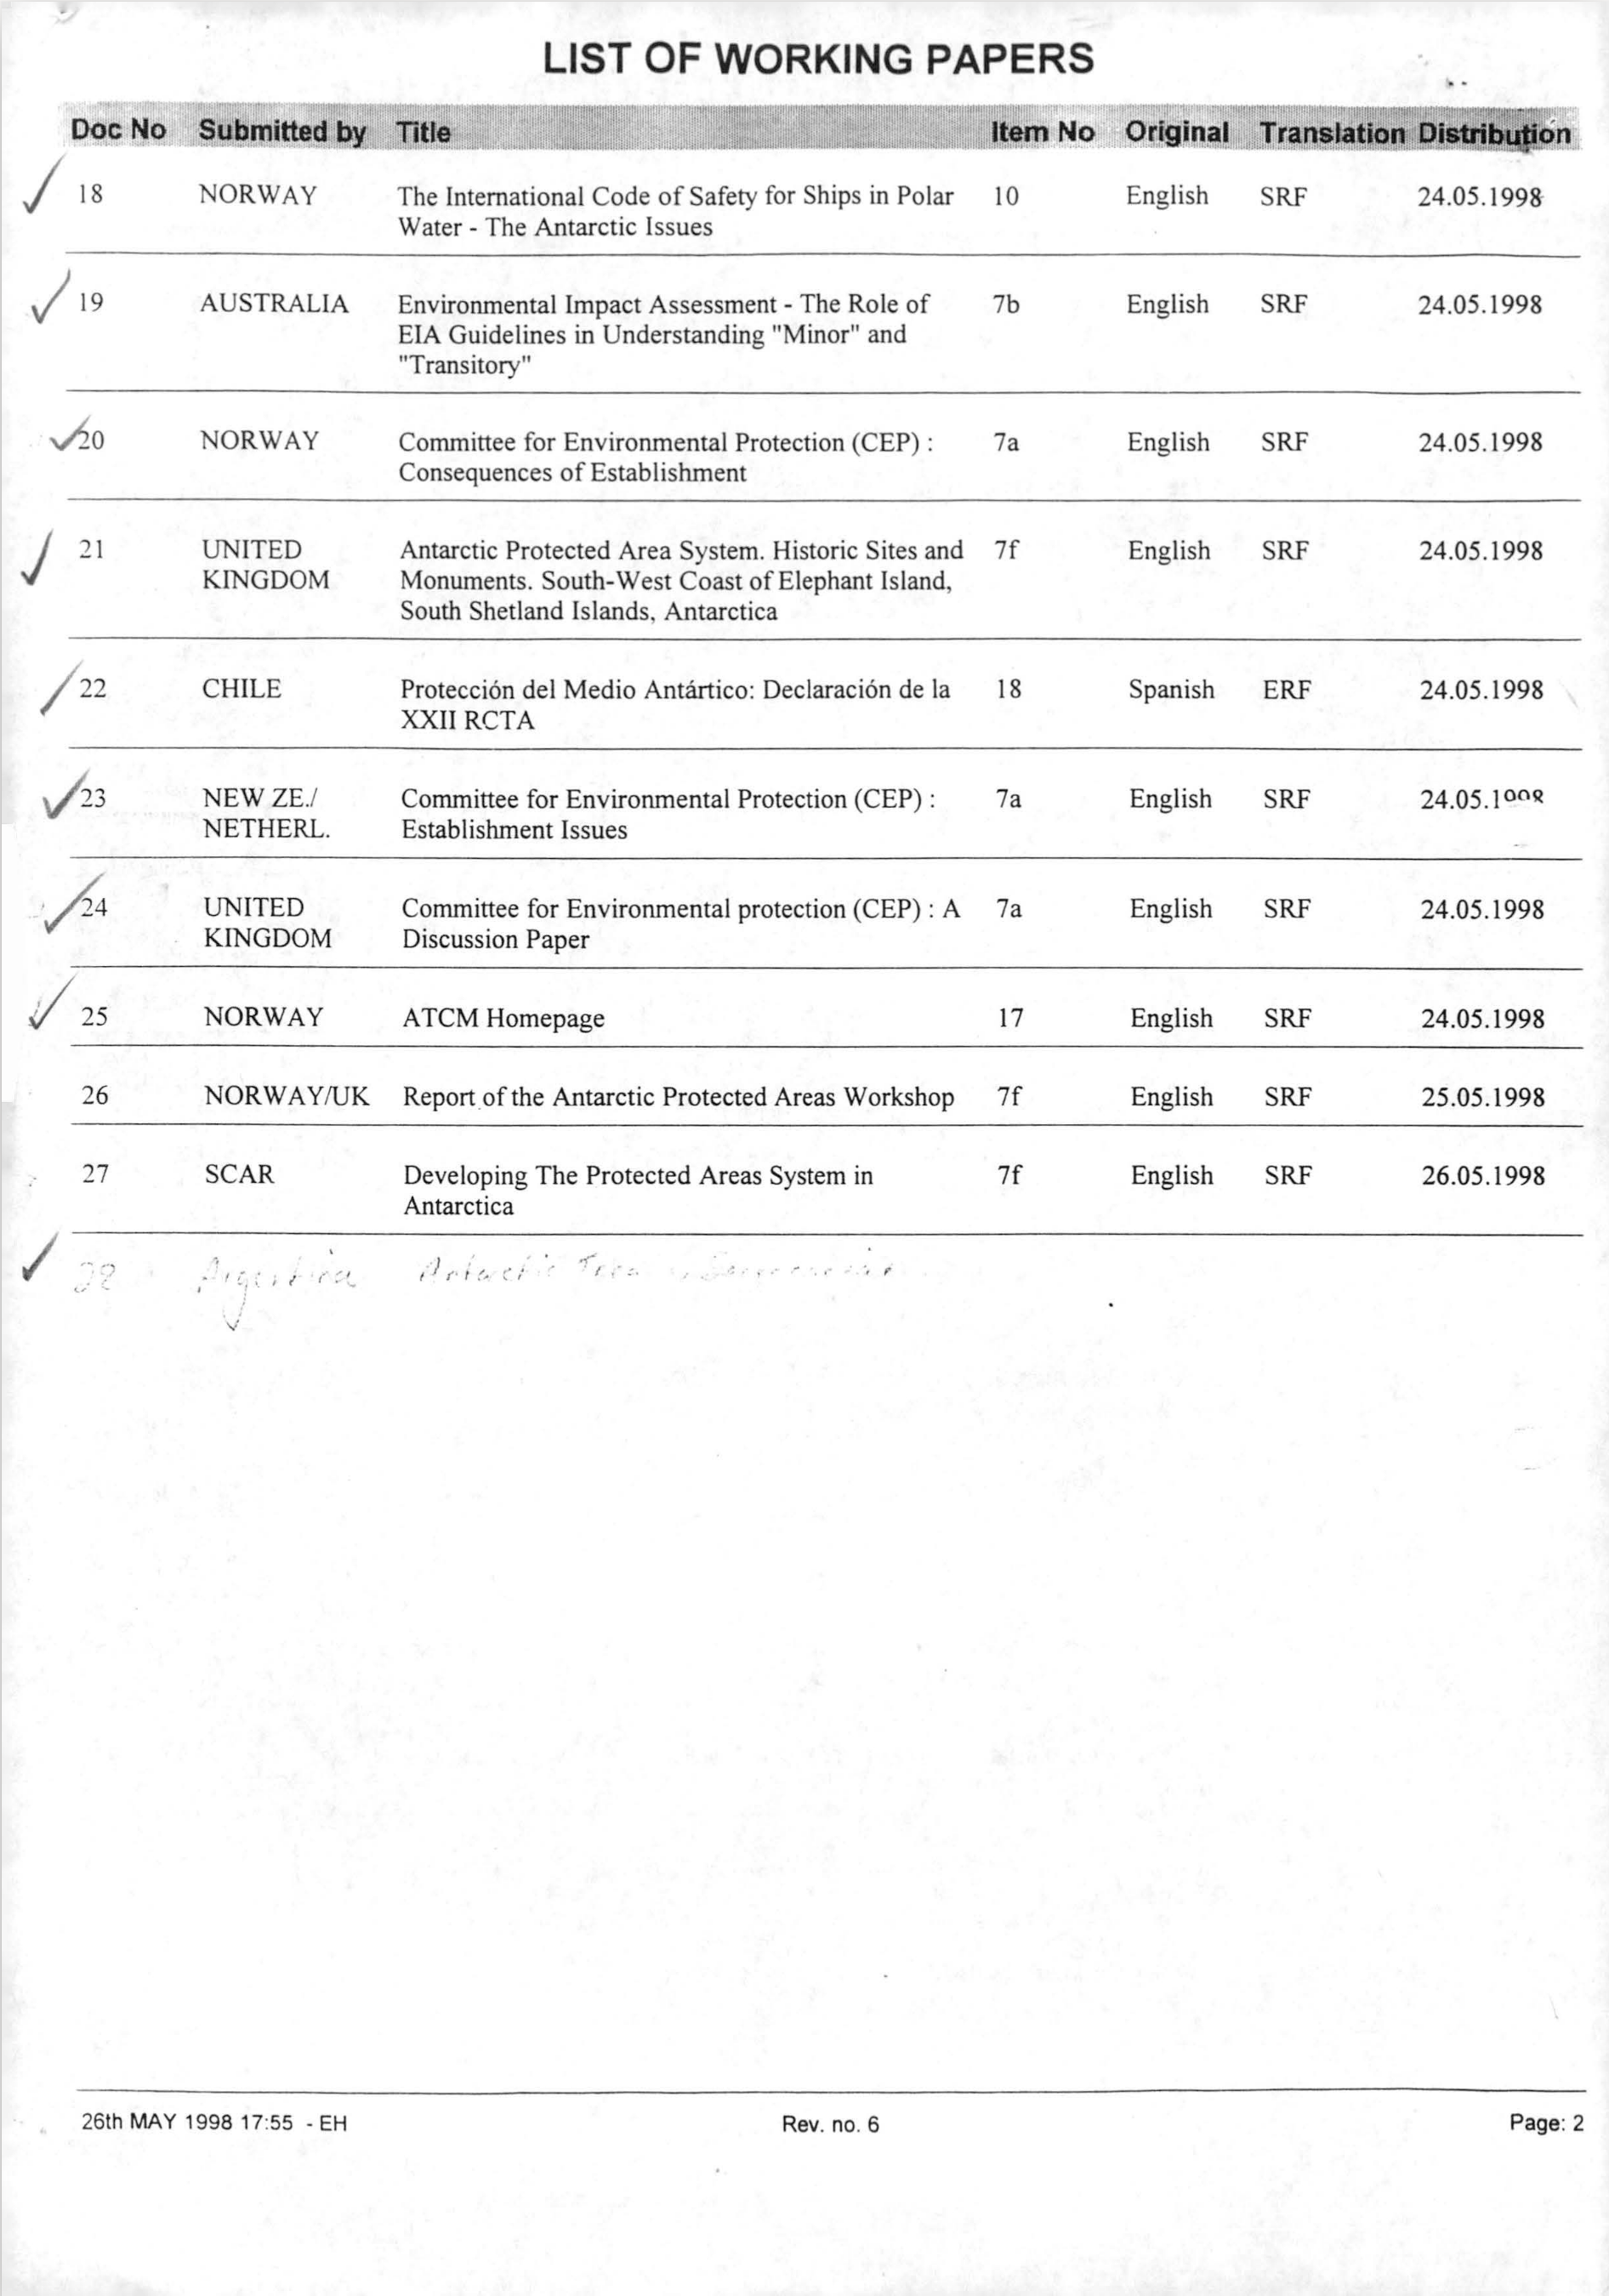
\includegraphics[width=\textwidth]{figures/bush_annotation.png}
    \end{minipage}
\end{figure}


\subsection{Text extraction}

\subsubsection{Determination of text-extraction method}

For each of the four document formats we encountered,
we used a different approach to extract their text:
\begin{enumerate}
    \item {\bf DOC}: A proprietary binary file format used by Microsoft Word versions 97-2003, storing text, formatting, and objects in a complex binary structure.

    {\bf Method}: DOC files were processed using a custom Python microservice (found in the {\tt pymupdf-microservice} directory) 
    that uses LibreOffice for conversion and text extraction.
    \item {\bf DOCX}: An XML-based file format introduced with Microsoft Word 2007, using compressed ZIP architecture to store document content, formatting, and metadata in separate XML files.

    {\bf Method}: Text was extracted directly from the XML structure within DOCX files, accessing the {\tt document.xml} component which contains the main content, 
    using PyMuPDF to process and normalise the extracted text.
    \item {\bf PDF with embedded text}: Documents containing machine-readable text that can be directly extracted, searched, and copied; typically created digitally through word processors, export functions, or digital printing.

    {\bf Method}: PyMuPDF's text extraction engine was used to directly access the embedded text layer. 
    \item {\bf PDF of scanned images}: Documents created by scanning physical papers, containing only image data without embedded text layers. 
    
    {\bf Method}: Optical Character Recognition (OCR) to convert the visual text into machine-readable format
    using a multimodal large language model (detailed below).
\end{enumerate}

To identify which PDFs required OCR processing,
we used a conservative heuristic approach.
Our system analysed each PDF using the PyMuPDF library (via the {\tt analyse\_image\_data()} function) 
to determine whether it contains actual text or merely scanned images.
For each page within the document, we calculated two metrics:
(1) the area coverage ratio, measuring what percentage of the page is covered by images;
and (2) the aspect ratio difference, comparing the image's dimensions with the page's dimensions to determine if they match.
If any page within the document contained an image that
covered more than 60\% of the page area and had an aspect ratio similar to the page's aspect ratio 
(with less than 35\% difference),
then the entire document was classified as a scanned document requiring OCR processing. 
This approach ensured that mixed documents (containing both text-based pages and scanned pages) were properly processed, 
as any presence of scanned content triggered the OCR workflow for the complete document.

The OCR pipeline was designed for robustness and resilience
so it could be stopped at any point in the process 
and would correctly resume from where it left off without duplicating work.
This was achieved through a dedicated SQLite database ({\tt document-pipeline.sqlite3}) 
that persistently tracked processing state of each document and page throughout the workflow.
We implemented transactional database operations to ensure atomic updates,
so each OCR operation either completes fully or rolls back entirely, with a precise timestamp recorded for provenance.
The system tracks each document page's status ({\tt 'extracted'} or {\tt 'ocr-done'}) in the database, 
allowing the OCR process to be stopped and resumed at any time without reprocessing already completed pages.
The pipeline also supports multiple OCR services (NVIDIA or Anthropic), 
allowing future workers to choose the most appropriate service based on document characteristics 
or to switch services if one becomes unavailable.
For services with size limitations (like Anthropic), 
the system intelligently downsamples images from 300 DPI to 150 DPI or even 100 DPI when necessary, 
maximising text recognition quality while staying within API constraints.
Parallel processing was implemented with controlled rate limiting, 
to process multiple pages simultaneously while respecting API limits to prevent overwhelming external services.
Each processing step is logged with detailed timing metrics and contextual information, 
creating a complete audit trail for diagnostics and performance analysis.
This architecture ensured that even for large-scale processing tasks that might take days to complete, 
the system could be paused, restarted, or even migrated between compute nodes without risk of data corruption or duplicate
processing, significantly enhancing the reliability of our OCR workflow for scientific research.

\subsubsection{Optical Character Recognition}

To perform OCR on scanned PDFs, 
we employed Meta's Llama-4-Maverick-17B-128E-Instruct model running on NVIDIA's cloud infrastructure. 
This model utilises a mixture-of-experts (MoE) architecture comprising 128 expert neural networks,
which specialise in different aspects of the input data
({\m cite: \url{https://ai.meta.com/blog/llama-4-multimodal-intelligence/}})
The `instruct' designation indicates that the model has undergone specialised fine-tuning to follow human instructions. 

We selected this model for the OCR task due to its native multimodal capabilities, 
which enable it to simultaneously process visual layout cues (such as formatting, tables, and positioning) alongside textual content. 
This integrated approach, combined with the model's large context window and robust instruction-following abilities, 
allows for accurate extraction and formatting of text from complex document layouts, 
effectively handling the nuanced visual and textual cues present in scanned materials.

The prompt used was as follows:
{\small 
\begin{verbatim}
    You are a precise OCR system. Your only task is to extract text from this image 
    with exact fidelity. Instructions:
    - Extract ALL text from the image with perfect accuracy
    - Maintain exact spacing and line breaks as they appear
    - If you can't read a character with certainty, represent it with [?]
    - If text is arranged in columns, preserve the column structure
    - Preserve any bullets, numbering, or indentation
    - For tables, use plain text formatting with spaces to align columns
    - Do not add ANY explanatory text, headers, or comments
    - Do not describe the image or its content
    - Return ONLY the extracted text
    - This is your input image: ...
\end{verbatim}
}

\section{Data description}

\subsection{Access}

\begin{itemize}
    \item For workers interested in the extracted texts only,
    the archive can be downloaded from {\m github repo}
        \begin{itemize}
            \item The texts are in the {\tt data\_doc\_texts/} directory
            \item Texts from ATADD and ATSD are split into 
            directories
            {\tt atadd\_utas\_database} and {\tt atsd\_secretariat\_database},
            respectively
            \item Summary figures describing the data (as used in this document)
            may be found in the {\tt results\_describe\_data} directory,
            \item Basic data accountability data is available in {\tt data\_accountability}
        \end{itemize}
    \item The full archive and data accountability can be downloaded from {\m Carlo's repo}.
    This archive includes source code used to identify documents in the ATSD, 
    extract the texts, and the full HTTP response cache.
    {\m need to coordinate with Carlo to fill this section out correctly}
\end{itemize}

\clearpage
\subsection{Data summary}

The textual content from 2469 WPs and 3875 IPs
was successfully extracted (Table~\ref{data_summary}).
Seven server errors occurred accessing the ATSD (HTTP 302).
%\begin{enumerate}
    %\item \url{https://documents.ats.aq/ATCM12/ip/ATCM12_ip010_e.pdf}
    %\item \url{https://documents.ats.aq/ATCM27/ip/ATCM27_ip025_e.doc}
    %\item \url{https://documents.ats.aq/ATCM27/ip/ATCM27_ip092_e.doc}
    %\item \url{https://documents.ats.aq/ATCM25/ip/ATCM25_ip009_e.pdf}
    %\item \url{https://documents.ats.aq/ATCM13/wp/ATCM13_wp013_s.pdf}
    %\item \url{https://documents.ats.aq/ATCM18/wp/ATCM18_wp005_e.pdf}
    %(note, however, revision 1 of this document was found)
    %\item \url{https://documents.ats.aq/ATCM25/wp/ATCM25_wp048_e.pdf}
%\end{enumerate}
The number of papers processed (6413) is higher than the number of
document files processed (6413) because 
5 document files downloaded from ATADD contained multiple revisions 
in the same WP in a single PDF.
Included in the `unusable papers' category
are documents that consisted only of only a title, 
a title page,
or referred to the content of the paper being available elsewhere.

\begin{table}[h]
    \centering
    \caption{Data summary (details in {\tt results\_describe\_data/annotate\_issues.csv}).}
    \label{data_summary}
    \begin{tabulary}{\textwidth}{LR}
        \toprule
        Data category & Nbr. \\
        \midrule
        Document URLs visited & 6415 \\
        Server errors & 7 \\
        Document files processed & 6408 \\
        Papers (WPs, IPs, and revisions) processed & 6413 \\
        \midrule
        Unusable papers & 69 \\
        \phantom{space} Paper withdrawn / number not used & 9 \\
        \phantom{space} Paper content missing & 60 \\
        \phantom{space space} File corrupted & 3 \\
        \phantom{space space} Text extraction failed & 12 \\
        \phantom{space space} Title or title-page only / text refers to content elsewhere & 45 \\
        \midrule
        Usable papers & 6344 \\
        \phantom{space} Usable WPs & 2469 \\
        \phantom{space} Usable IPs & 3875 \\
        \bottomrule
    \end{tabulary} 
\end{table}

% \subsection{Extraction method summary}

The extraction technique used varied with publication date
(Fig.~\ref{extraction_method_v_year_combined}).
Early PDFs were processed with AI,
more recent PDFs with PyMuPDF,
DOCs were most common between 2002 and 2020,
and papers within the last 4 years were DOCXs.
Of the 6413 papers processed, 
2082 were PDFs using AI (1171 WPs and 911 IPs),
341 were PDFs using PyMuPDF (92 WPs and 249 IPs),
3141 were DOCs using LibreOffice (978 WPs and 2163 IPs),
and 849 were DOCXs using PyMuPDF (243 WPs and 606 IPs)
(details in {\tt results\_describe\_data/which\_OCR\_with\_AI.csv}).

\begin{figure}[h]
    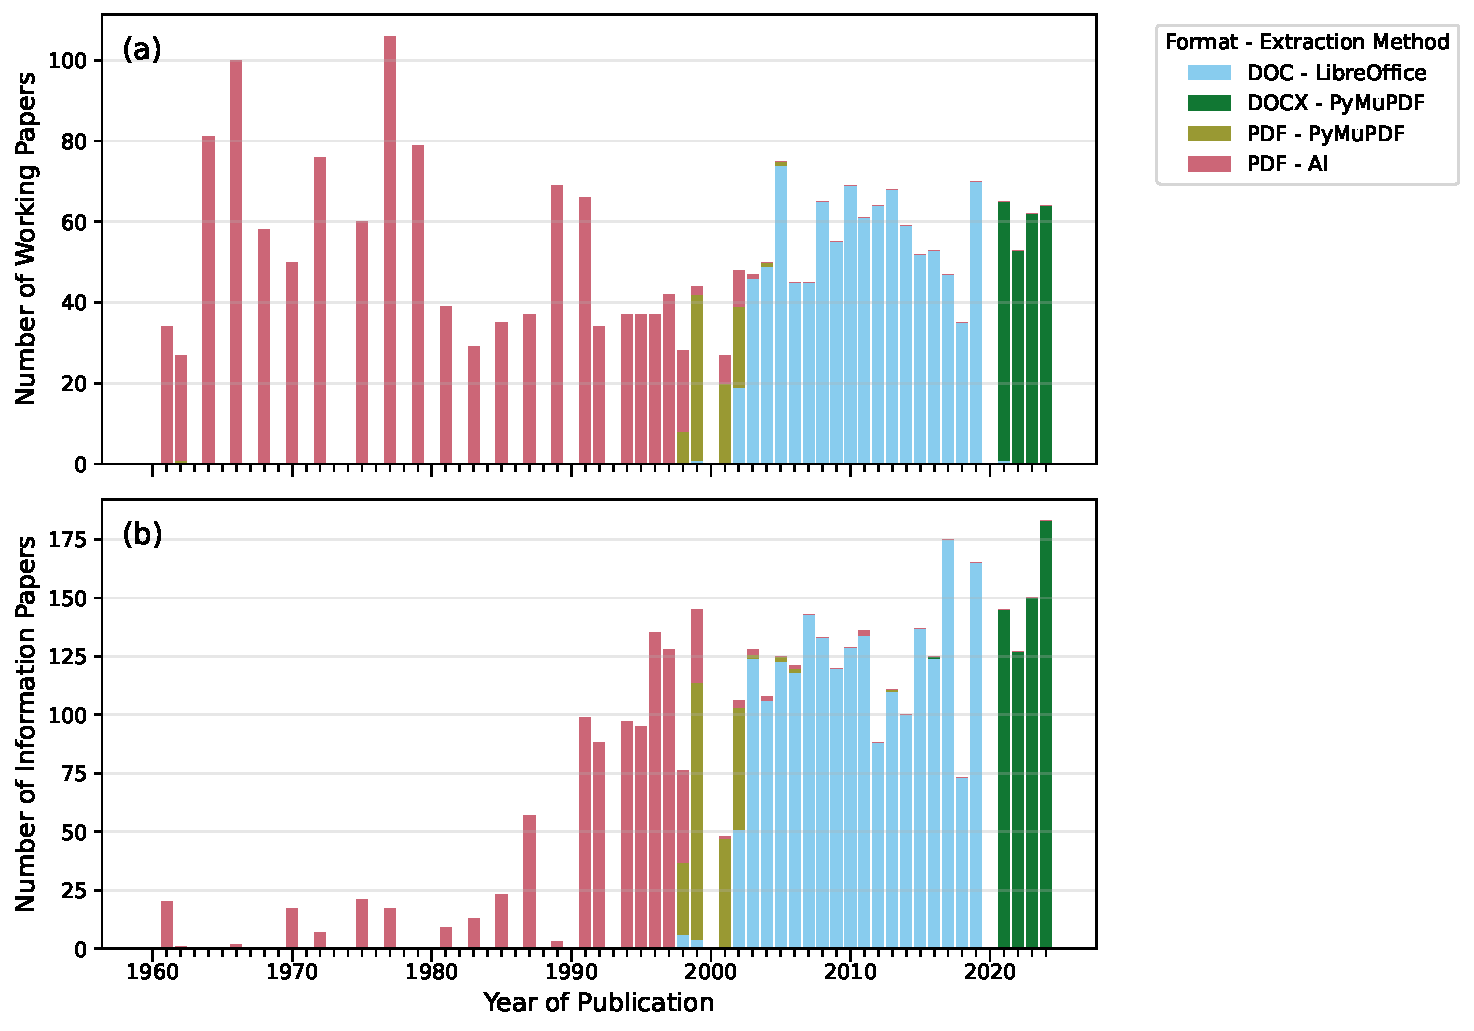
\includegraphics[width=\textwidth]{../results_describe_data/extraction_method_v_year_combined.pdf}
    \caption{
        The number of (a) Working Papers and (b) Information Papers
        extracted by year of publication.
        Data includes unsuccessful extractions (e.g., file corrupted).
    } \label{extraction_method_v_year_combined}
\end{figure}

\newpage
Extracted-text coverage was lower in IPs than WPs,
with missing IPs clustered in certain years
(Fig.~\ref{coverage_v_year_combined}).
The existence of `potentially missing' papers was
inferred by gaps in the paper-numbering sequence
(total: 218 papers).
It should be noted, therefore,
that estimates of `potentially missing' IPs could 
not be made for years with no IPs.
`Definitely missing' papers are papers whose existence is known
(e.g., from official document lists)
but the text is not available (total: 78).
A paper could be `definitely missing'
because: 
the paper could not be downloaded, i.e., server error;
the file was corrupted; 
the text-extraction failed;
the original paper was missing content, e.g., only contained the title page;
or the original paper indicated that the content was available elsewhere,
e.g., distributed separately or available as an attachment.
As detailed below,
some papers were tagged with the wrong language
or contained a mix of languages.
Therefore,
the language indicated in Fig.~\ref{coverage_v_year_combined} 
is only the tagged language if that language was present in the text;
otherwise, the majority language detected by counted dictionary-recognised words was used.

\begin{figure}[h]
    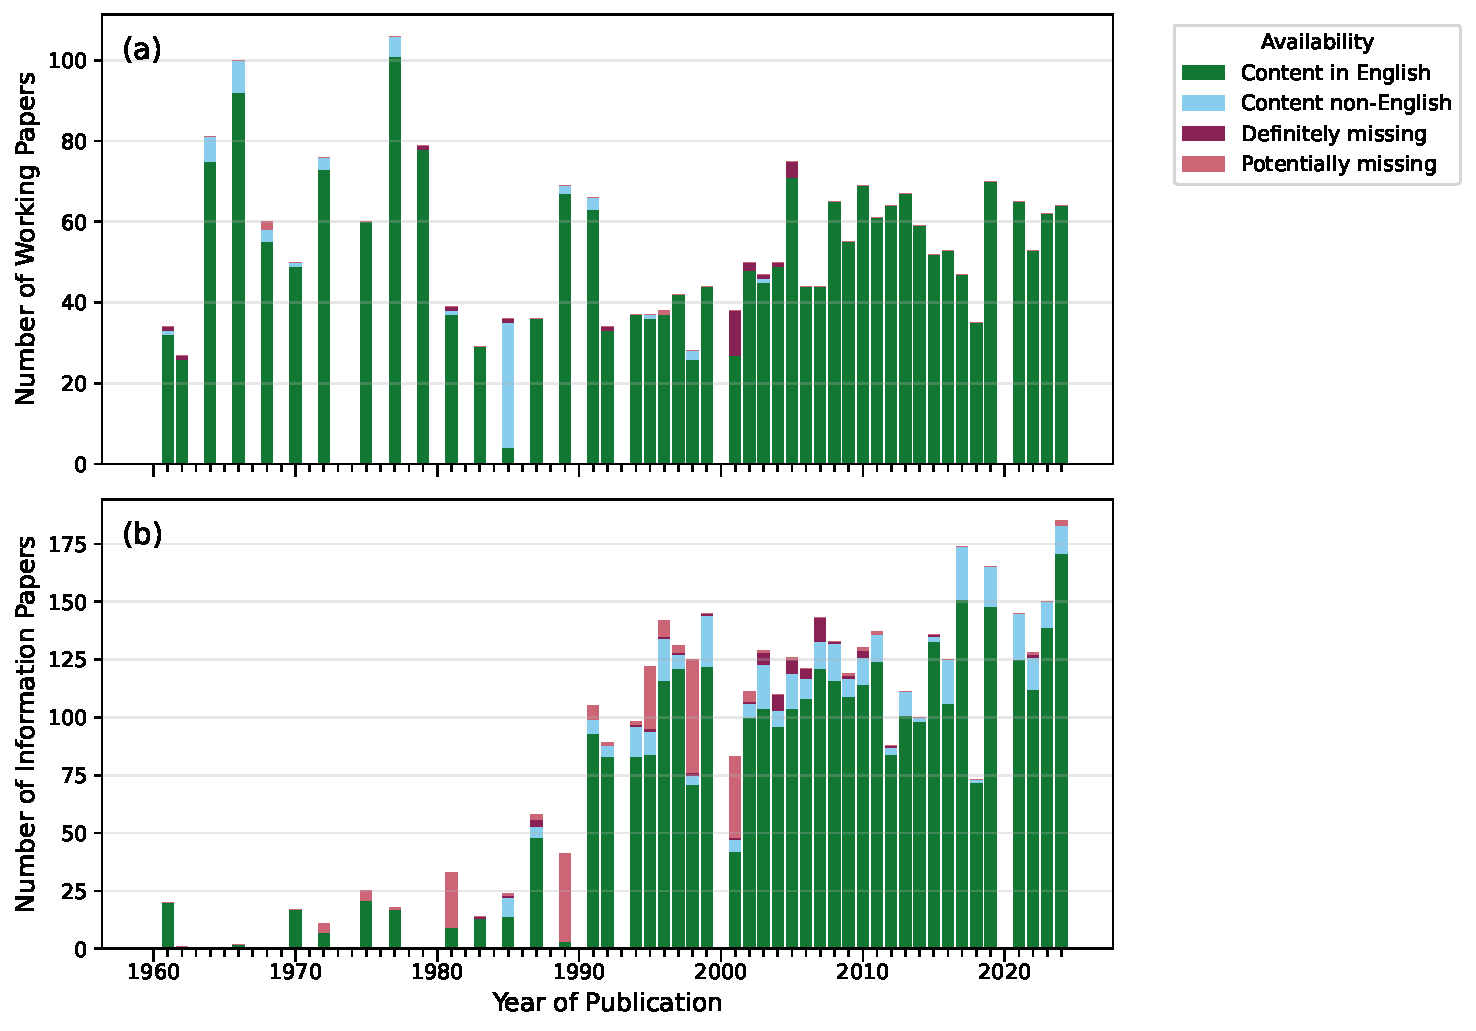
\includegraphics[width=\textwidth]{../results_describe_data/coverage_v_year_combined.pdf}
    \caption{
        Text coverage over time.
        The language was determined from either the tagged language 
        (if language present in paper)
        or the majority language detected.
        `Definitely missing' are papers 
        whose existence is known
        but the content text was not extracted,
        and `potentially missing' papers 
        were inferred from gaps in the paper-numbering
        sequence (see Sect.~\ref{S:data_limitations}).
    } \label{coverage_v_year_combined}
\end{figure}

\clearpage
\subsection{Data limitations}
\label{S:data_limitations}

\subsubsection{Corrupted files and failed text extractions}

To identify corrupted files and failed extractions,
we ordered extracted texts by their number of words extracted,
and texts up to 115 words were manually checked.
The cut-off of 115 words was chosen based on the plateau
in the cumulative number of texts found with missing content
(Fig.~\ref{missing_content}).
For texts with missing content with no explanation
(e.g., the text indicated the document had been withdrawn
or content was available as an attachment),
the original document file was checked.

\begin{figure}[h]
    \begin{minipage}[b]{0.40\textwidth}
        \caption{
            With paper texts indexed in order of increasing number of words,
            the manual-check cut-off (115 words),
            and (inset) the cumulative number of texts with missing content.
            Missing content includes texts that were empty
            or that consisted of a title or title-page only,
            but excludes texts that referred to documents 
            available as attachments or circulated separately.
        } \label{missing_content}
    \end{minipage}
    \hfill
    \begin{minipage}[b]{0.55\textwidth}
        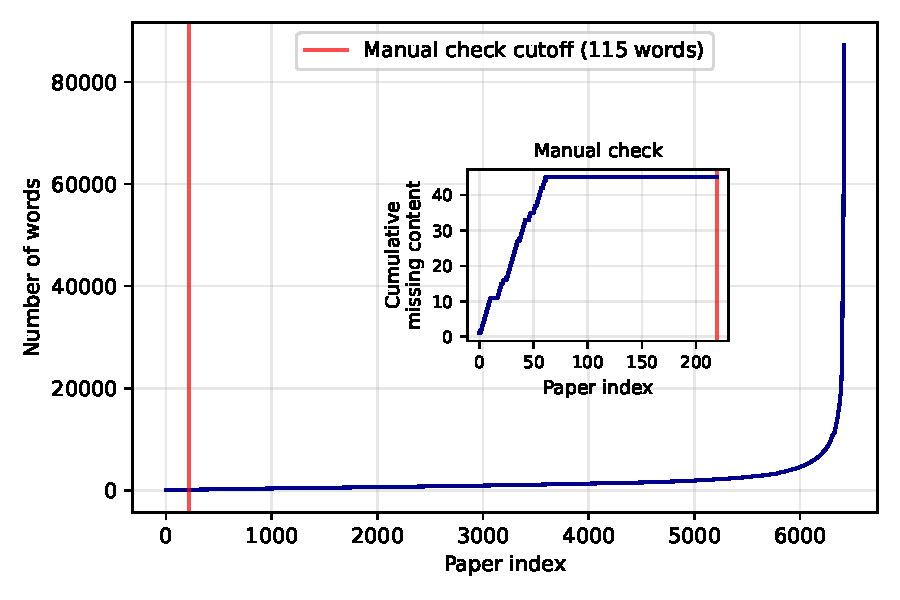
\includegraphics[width=\textwidth]{../results_describe_data/missing_content.pdf}
    \end{minipage}
\end{figure}

Of the 45 extracted texts with missing content,
3 were found to be the result of corrupted original files
and 12 were the result of failures in the text extraction.
Of the 12 failed extractions,
3 were failed AI extractions,
2 were failed of PyMuPDF extractions,
and 7 were failed LibreOffice extractions
(details in {\tt results\_describe\_data/check\_missing\_content.ods}).
The failed AI extractions were
poorly scanned (though legible) typewritten documents from ATCMs 1 and 2.
The cause of the PyMuPDF extraction failures was unclear.
LibreOffice typically failed on DOCs where 
the document text content was embedded in text boxes.

\subsubsection{Dictionary check of extracted texts}

To check for intelligibility trends with publication date,
we investigated how the proportion of unknown words 
varied with time. 
Unknown words were words that were not recognised by any of the 
dictionaries in the four languages (English, Spanish, French, Russian).
This metric was applied to all texts regardless of their
tagged language to account for mistagged papers and papers
containing a mix of languages (see below).

The proportion of unknown words 
has a U-shaped relationship with publication date,
with an initial decline until the 1980s followed by increase and levelling off
(Fig.~\ref{propn_unknown_words_v_year_two_panel_annotate}).
A high proportion of unknown words was not indicative of text-extraction problems.
Each extracted text with proportion $> 0.15$ unknown words was manually checked,
and in all cases the high proportion was attributable to correctly
extracted content such as names, places, and technical terms
({\tt results\_describe\_data/problematic\_language\_length.csv}).
IPs in later years had a higher proportions of unknown words
due to their technical content.
For example,
the paper with the highest proportion of unknown words
(ATCM 45, IP 103) contained lists of taxonomic names 
and abbreviations.

\begin{figure}[h]
    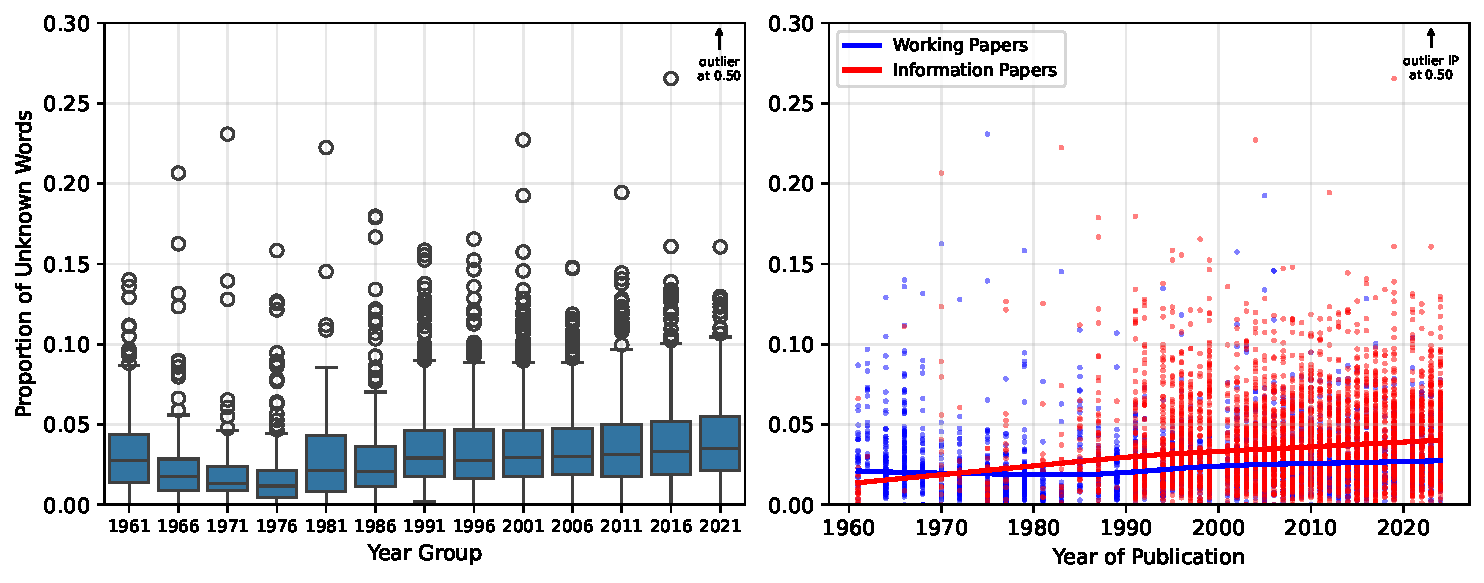
\includegraphics[width=\textwidth]{../results_describe_data/propn_unknown_words_v_year_two_panel_annotate.pdf}
    \caption{
        Proportion of unknown words
        (words unknown to the four language dictionaries:
        English, Spanish, French, and Russian)
        per document.
        These data exclude documents known to have missing content,
        to have been withdrawn, or content elsewhere.
    } \label{propn_unknown_words_v_year_two_panel_annotate}
\end{figure}

\subsubsection{Illegible characters}

To estimate illegibility rates,
we combined the AI's self-reported performance with heuristics
and manual checking.
The AI prompt included an instruction to 
insert a {\tt [?]} into the text for any illegible characters;
however,
we found that the AI frequently frequently inserted {\tt ?} 
with no square brackets instead (e.g., Fig.~\ref{compare_methods}c).
Therefore,
a heuristic was needed to distinguish between AI-inserted illegibility markers
and question marks present in the original text.
Likely illegibility markers were identified by 
searching for a {\tt ?} character that occurred
within alphanumeric sequences, 
at the start of a word followed by letters, or in sequence.
In addition, up to 50 examples of words containing each type of illegibility
marker were extracted and tabulated alongside the 
illegible-character counts for faster checking
({\tt results\_describe\_data/count\_illegible\_ocr.csv}).
The table was analysed by hand
with manual checking of the text files and original documents where needed
({\tt results\_describe\_data/count\_illegible\_ocr\_by\_hand.csv}).
To obtain a conservative overestimate
of self-reported illegible-character percentages,
we excluded documents with {\tt ?} characters that did \emph{not} indicate
illegibility (column: {\tt determination\_by\_human}).

\begin{figure}[h]
    \begin{minipage}[b]{0.30\textwidth}
        \caption{
            Example comparing methods: (a) original text,
            (b) Linux tools ({\tt pdfsandwich} followed by {\tt pdftotext -layout}),
            and (c) our AI method.
            To improve visual comparison,
            extracted texts were manually indented
            and extra whitespace produced by the Linux-tools method was deleted.
            It is interesting to note that the second error in (c) 
            corrects a grammatical error made in the original text.
            Taken from page 2 of ATCM 11 WP19.
        } \label{compare_methods}
    \end{minipage}
    \hfill
    \begin{minipage}[b]{0.65\textwidth}
        \begin{center}
            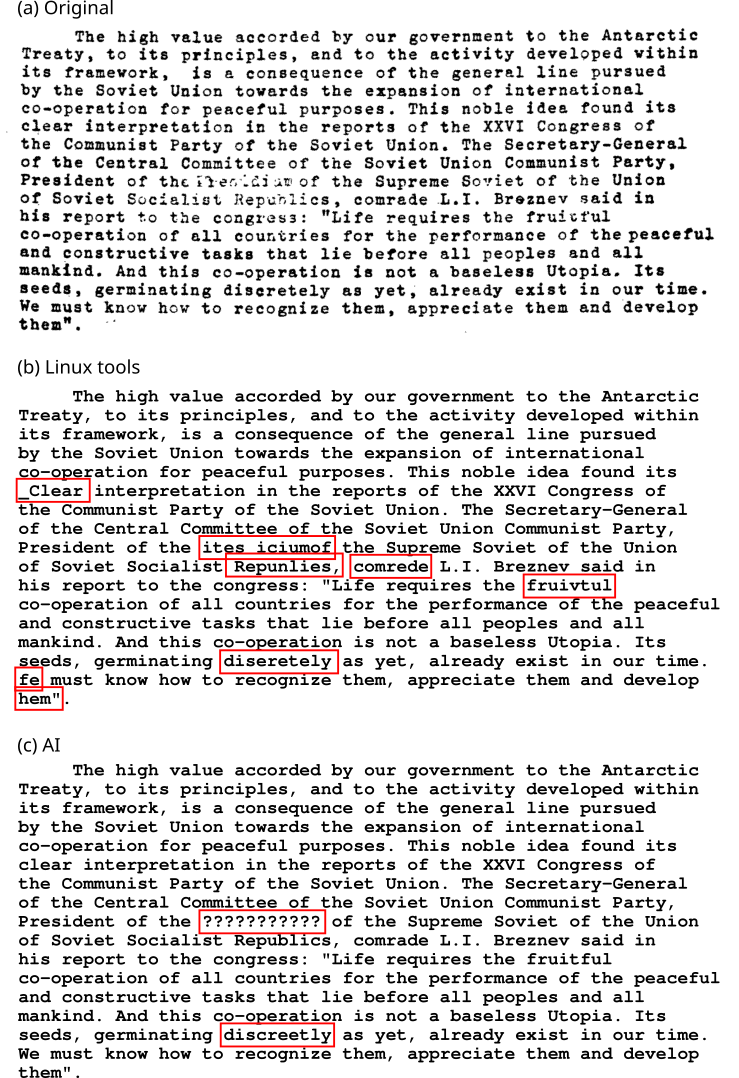
\includegraphics[width=\textwidth]{figures/compare_methods.png}
        \end{center}
    \end{minipage}
\end{figure}

\newpage
The percentage of illegible characters was higher in earlier years
(Fig~\ref{percentage_illegible_v_year}),
which was expected because early-year documents were typewritten
and document quality was poor.
A noticeable exception to the trend occurred in 1981,
where there is a spike in the percentage of illegible characters.
Through manual investigation,
we attribute this spike to two unusual documents in that year:
ATCM 11 IP2
had a large number of illegible characters in 
the footnotes to a data table in Spanish,
and ATCM 11 WP19 (page 2) had one whole word (potentially Russian)
illegible (Fig.~\ref{compare_methods}). 
Removing both of these documents reduces the 1981 illegibility
percentage to approximately one quarter, 
bringing it into agreement with percentages in nearby years.

\begin{figure}[h]
    \begin{minipage}[b]{0.40\textwidth}
        \caption{
            Percentage of characters marked illegible by the AI
            in relation to year of publication.
            Note that the percentages given are over-estimates
            (see text).
        } \label{percentage_illegible_v_year}
    \end{minipage}
    \hfill
    \begin{minipage}[b]{0.55\textwidth}
        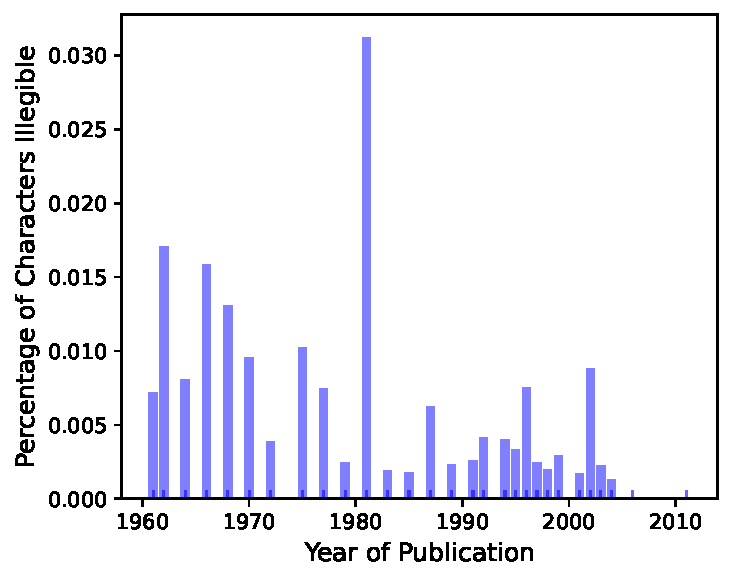
\includegraphics[width=\textwidth]{../results_describe_data/percentage_illegible_v_year.pdf}
    \end{minipage}
\end{figure}

\newpage
\subsubsection{Cross-validation with Linux-tool OCR}

{\m TO DO}

\begin{itemize}
    \item {\tt pdfsandwich} \citep{pdfsandwich} 
    and {\tt pdftotext -layout} \citep{pdftotext}
    \item text alignment with {\tt difflib}
\end{itemize}

\clearpage
\subsubsection{Language mislabelling}

To identify papers mistagged with the wrong language,
we ordered extracted texts by their proportion of 
non-tagged-language words,
and texts with high proportions were manually checked.
Specifically, we calculated the proportion of 
words that were not recognised by the tagged-language dictionary 
but were recognised by an other-language dictionary.
The manual checks were performed for all extracted texts with
proportion $\geq 0.07$,
where this cut-off was chosen based
on the plateau in the cumulative number of 
mistagged texts found (Fig.~\ref{language_mistagged}).

Due to the presence of mixed-language papers in the corpus,
a strict definition of language mistagging was employed;
a paper was considered mistagged if none of the content was 
in the tagged language.
Therefore, papers that contained a mix of languages 
and were tagged with one of those languages were not considered mistagged
(e.g., ATCM 5 WP23 includes a summary translated into each of the four languages,
while the main content is in English).
Future researchers should consult
{\tt results\_describe\_data/problematic\_language\_length.csv}
to determine which documents are suitable to their needs.
The dictionaries used to identify words were employed using {\tt PyEnchant} 
\citep{pyenchant, enchant}.
The English-language dictionaries used were 
{\tt en\_US} and {\tt en\_GB} from Aspell \citep{aspell},
the non-English dictionaries were
{\tt es\_ES}, {\tt es\_MX}, {\tt es\_AR}, {\tt fr\_FR}, and {\tt ru\_RU}
from Hunspell \citep{hunspell}.

\begin{figure}[h]
    \begin{minipage}[b]{0.40\textwidth}
        \caption{
            With paper texts indexed in decreasing order of 
            proportion of non-tagged-language words,
            the manual-check cut-off (proportion $= 0.07$)
            and (inset) the cumulative number of 
            mistagged texts found.
            Mistagged texts contained no content in the tagged language.
        } \label{language_mistagged}
    \end{minipage}
    \hfill
    \begin{minipage}[b]{0.55\textwidth}
        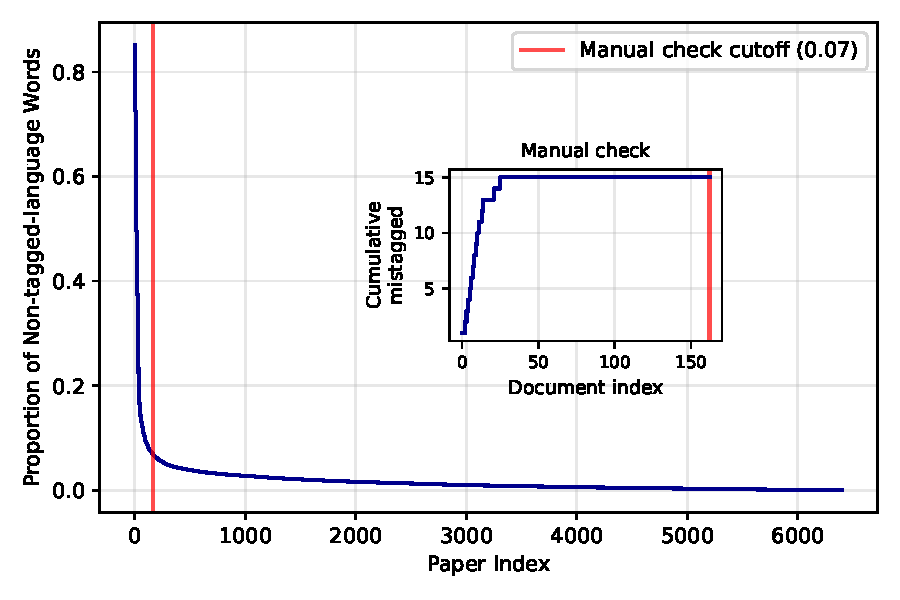
\includegraphics[width=\textwidth]{../results_describe_data/language_mistagged.pdf}
    \end{minipage}
\end{figure}


\section{Discussion and recommendations for future work}

\begin{itemize}
    \item first para 2 points:
    \begin{itemize}
        \item Quick one-or-two-sentence summary of what we did
        \item Say we hope that the dataset
        will provide a baseline upon which future researchers will contribute
        their own refinements
        \item Segue sentence saying we'll now talk about main shorcomings
    \end{itemize}
    \item Ways to address missing content
    \begin{itemize}
        \item Some attachments, particularly for IPs, may be available in ATSD
        as a downloadable attachment.
        See {\tt results\_describe\_data/check\_missing\_content.ods} 
        and {problematic\_language\_length.ods} for candidates.
        \item The same process we used to ID missing WPs could be used for IPs;
        namely, find paper-numbering sequence gaps, consult lists of documents.
        We've made a start for WPs.
        \item Translation of non-English documents
    \end{itemize}
    \item Structural information missing (sections) and handling of tables and figures
    \begin{itemize}
        \item Our primary concern was extraction of words only for NLP
        \item Encoding to Markdown or other format might be used to 
        preserve document structure
        \item Can AI handle tables into Markdown?
        \item Identification of figures and extract as image files
    \end{itemize}
    \item Future workers should learn from our fail regarding the square-bracketed
    question-mark instruction
    \item Final reports could also be done using the same approach
\end{itemize}

\section{Conclusion}

\begin{itemize}
    \item We have provided a dataset and we made our methods available
    on the Github collaborative platform,
    and we invite future workers to contribute to and improve upon the work.
    \item Say something nice about the ATS and its uniqueness;
    unique ecosystem, unique global cooperation (for peaceful purposes only)
    \item We hope that our methods and data will be useful to future workers
    towards both safe-guarding Antarctic ecosystems 
    and learning from the global scientific and political cooperation that has 
    been begun there.
\end{itemize}

\section{Acknowledgements}

Nvidia; Zach's funder

% ---------------------------------------------------------------------------------------
\bibliographystyle{dcu}
\bibliography{ats.bib}
% ---------------------------------------------------------------------------------------
\end{document}
